
\section{Aufgabe 4.2}


\subsection{Spurious states}

In diesem Aufgabenteil sollten für zufällige Neuronenkonfigurationen die Anzahl der \textbf{spurious sates} in Abhängigkeit von $p/N$ gezählt werden. Dabei wurde eine Fehlerrate unter 5 Prozent als Konvergenz zu einem gespeicherten Bild gezählt. Außerdem wurde auch das negative Bild $\xi_i^{(\mu)}$ gezählt. Die Wahrscheinlichkeit in ein spurious state zu konvergieren $P(\textup{spurious states})$ wurde in Abhängigkeit von $p/N$ in \autoref{fig:spurious_states_10000} geplotted. Hierbei wurde für jedes $p/N$ 100 verschiedene 100-Neuronen-Netzwerke mit jeweils 1000 verschiedenen Neuronenkonfigurationen gestartet.

\begin{figure}[htp]
	\centering
	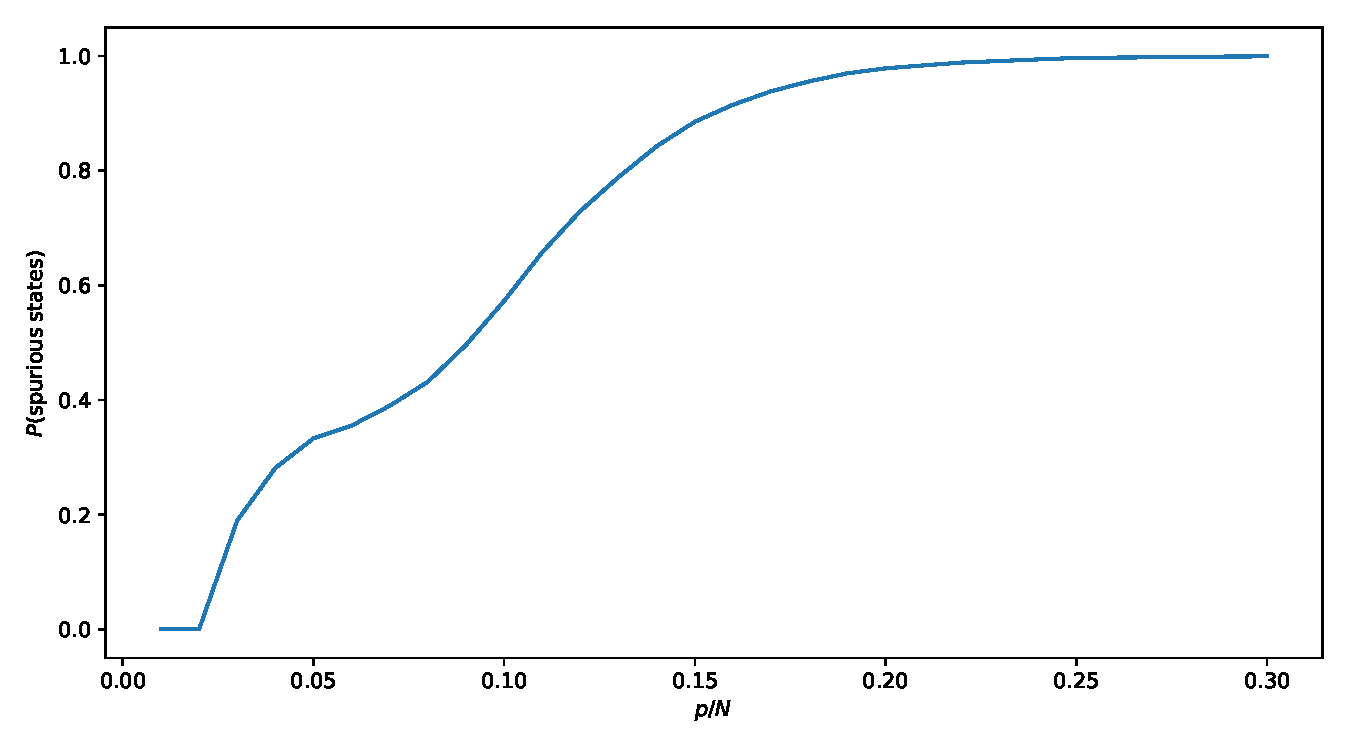
\includegraphics[width = \textwidth]{images/4_2_1/spurious_states_1000_1000.pdf}
	\caption{Wahrscheinlichkeit $P(\textup{spurious states})$ in ein spurious state zu konvergieren in Abhängigkeit von $p/N$.}
	\label{fig:spurious_states_10000}
\end{figure}

Wie zu erkennen, steigt mit zunehmender Anzahl gespeicherter Bilder auch die Wahrscheinlichkeit in ein spurious state zu konvergieren. Bei $p/N = 0.1$ liegt diese schon bei 50 Prozent und konvergiert ab etwa $p/N = 0.2$ gegen 100 Prozent. Dies lässt sich damit erklären, dass mit $p/N$ die Anzahl der Nebenminima steigt und somit der basin of attraction der gespeicherten Bilder verkleinert wird. Bei sehr großer Anzahl von Bildern sind  die gespeicherten Bilder selbst auch keine Minima mehr. Dies führt dazu, dass die Wahrscheinlichkeit zur Konvergenz in ein spurious state auf 100 Prozent steigt. Hierbei sei noch anzumerken, dass die genaue Form des Graphen natürlich von der willkürlichen Definition, wann ein Fixpunkt als spurious state zu zählen ist (hier über 5 Prozent Fehlerrate), abhängig ist.

Der Code zu Aufgabe 4.2.1 befindet sich in \textbf{aufgabe4\_2\_1.py}.

\subsection{Endliche Temperaturen}

In diesem Aufgabenteil sollten endliche Temperatur für $\beta < \infty$ so implementiert werden, dass die Tendenz zu den 'spurious states' abnimmt. Da bei endlichen Temperaturen keine exakte Konvergenz mehr einsetzt, muss ein anderes Abbrechkriterium gewählt werden. Um einen sinnvollen Vergleich zu dem Update ohne endliche Temperaturen zu ziehen sollten beide Varianten mit der selben Anzahl von Iterationen ausgeführt werden. Wie man in \autoref{fig:iterationen_fixpunkt} sieht, liegt die durchschnittliche Dauer bis zur Konvergenz bei maximal 12 Iterationen. Deshalb wurde entschieden die Fehlerrate nach 20 Iterationen zu messen, da somit nahezu sichergesellt ist, dass das Netzwerk ohne endliche Temperaturen in ein Fixpunkt konvergieren kann. Auch hier wurde eine Fehlerrate unter 5 Prozent als Konvergenz zu einem gespeicherten Bild gezählt.

Die Wahrscheinlichkeit in ein spurious state  $P(\textup{spurious states})$ nach 20 Iterationen zu erreichen wurde für verschiedene inversere Temperaturen $\beta$ in Abhängigkeit von $p/N$ in \autoref{fig:spurious_states_10000} geplotted. 

\begin{figure}[htp]
	\centering
	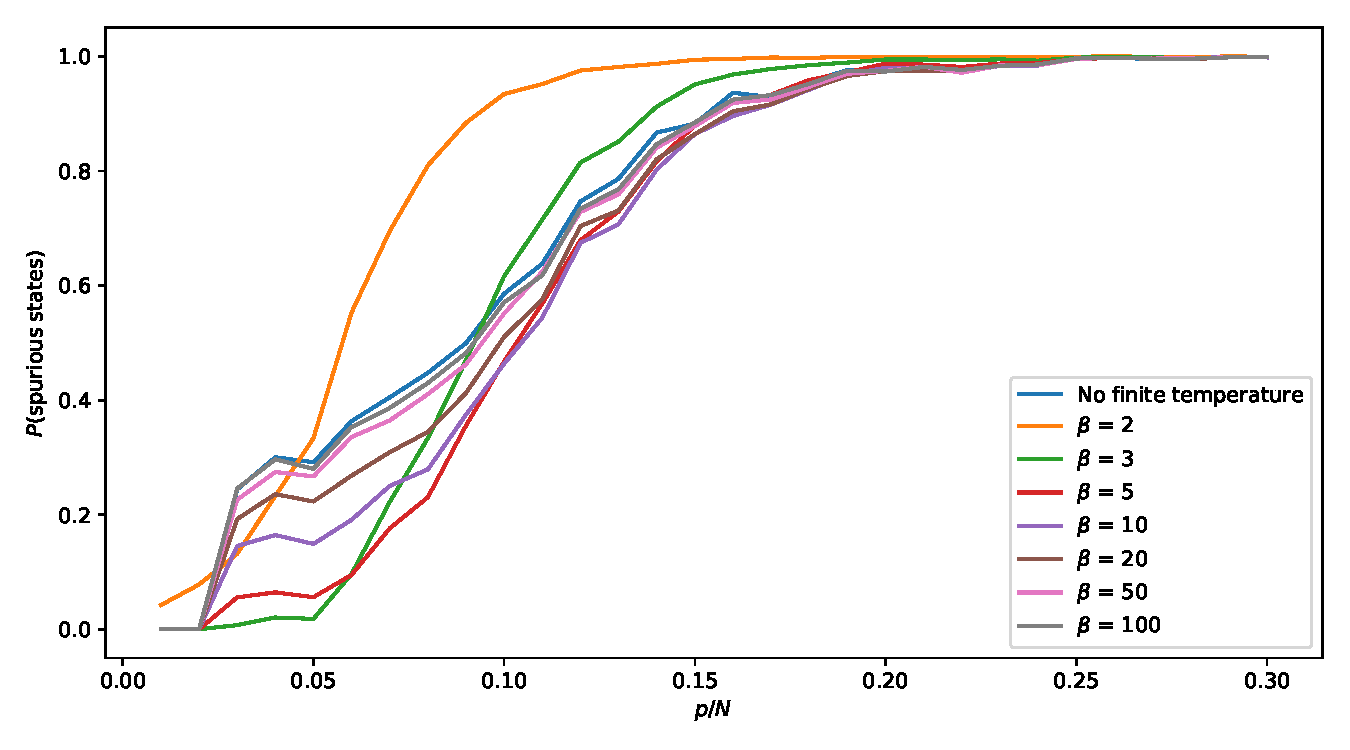
\includegraphics[width = \textwidth]{images/4_2_2/spurious_states_finite_temperature_100_100.pdf}
	\caption{Wahrscheinlichkeit $P(\textup{spurious states})$ in ein spurious state zu konvergieren in Abhängigkeit von $p/N$.}
	\label{fig:spurious_states_finite_temperature_100}
\end{figure}

Wie zu erkennen ist die Wahrscheinlichkeit in ein spurious state zu konvergieren für ein Update mit $\beta = 2$ für den Großteil der Verhältnisse $p/N$ deutlich größer als bei einem Update ohne endliche Temperaturen. Dies lässt sich damit erklären, dass die Fluktuationen noch zu stark sind. Für $\beta = 3$ ist die Wahrscheinlichkeit bis $p/N < 0.08$ schon deutlich unter der ohne endlicher Temperatur. Für $\beta = 3$ wird ein Optimum erreicht: Hier liegt die Wahrscheinlichkeit in ein spurious state zu konvergieren immer unter der ohne endliche Temperaturen. Bei $p/N =0.05$ beträgt diese bei etwa nur ein Zehntel und bei $p/N = 0.1$ bei immerhin noch 80 Prozent der des Updates ohne endliche Temperaturen. Für $p/N > 0.15$ sind beide identisch und konvergieren ab $p/N = 0.25$ gegen 100 Prozent.

Mit zunehmneden $\beta$ nähert sich der Verlauf der Wahrscheinlichkeit in ein spurious state zu konvergieren asymptotisch dem ohne endliche Temperaturen. Für $\beta = 100$ sind beide Verläufe nahezu identisch. Dies lässt sich noch einmal am Graphen der Sigmoid-Funktion

\begin{align}
P(S_i = \pm1) = \frac{1}{1 + exp(\mp2 \beta h_i)}
\end{align}

verdeutlichen (siehe \autoref{fig:sigmoid_finite_temperatures}): Für kleine $\beta$ ist der Graph relativ flach, was ein großen Fluktuation entspricht. Im Grenzfall $\beta \rightarrow 0$ wird das Update komplett zufällig. Im anderen Grenzfall $\beta \rightarrow 0$ wird die Sigmoid-Funktion zur Signum-Stufenfunktion, was der deterministischen McCulloch-Pitts Gleichung entspricht.

\begin{figure}[htp]
	\centering
	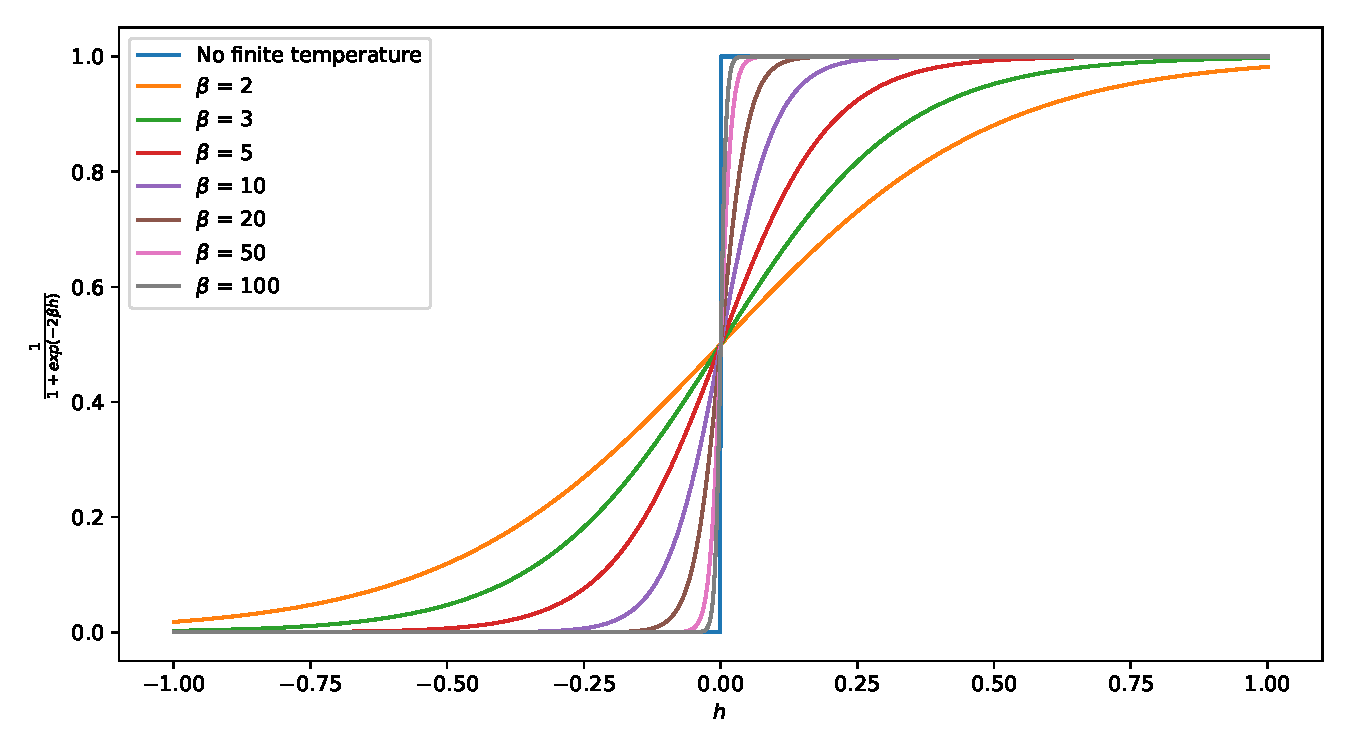
\includegraphics[width = 0.75\textwidth]{images/sigmoid_finite_temperatures.pdf}
	\caption{Die Sigmoidfunktion für verschiedene Werte von $\beta$.}
	\label{fig:sigmoid_finite_temperatures}
\end{figure}

Der Code zu Aufgabe 4.2.2 befindet sich in \textbf{aufgabe4\_2\_2.py}.














\clearpage
